\ifdefined\ishandout
\documentclass[handout]{beamer}
\else
\documentclass{beamer}
\fi

\usepackage[frenchb]{babel}
\usepackage[T1]{fontenc}
\usepackage[latin1]{inputenc}
\usepackage{hyperref}
\usepackage{multirow}
\usepackage{listings}
\usepackage{fancyvrb}
\usepackage{tikz}
\usepackage{framed}
\usepackage{algorithm}
\usepackage{algorithmic}
\usepackage{xcolor}
\usepackage{color, colortbl}
\usepackage{handoutWithNotes}
\usepackage{amsmath}
\usetikzlibrary{shapes.geometric}
\usetikzlibrary{positioning}
\usetikzlibrary{shapes.arrows, chains}
\usetikzlibrary{arrows,calc}
\usetikzlibrary{shapes.multipart}
\usepackage{array}
\usetheme{Boadilla}

\ifdefined\ishandout
\pgfpagesuselayout{3 on 1 with notes}[a4paper,border shrink=5mm]
\usecolortheme{dove}
\else
\usecolortheme{dolphin}
\fi


\lstnewenvironment{codeC}
{ \lstset{language=C,
    otherkeywords={printf,scanf}}
}
{}

\ifdefined\ishandout
\definecolor{mygreen}{rgb}{0,0,0}
\definecolor{mymauve}{rgb}{0,0,0}
\definecolor{myblue}{rgb}{0,0,0}
\else
\definecolor{mygreen}{rgb}{0,0.6,0}
\definecolor{mymauve}{rgb}{0.58,0,0.82}
\definecolor{myblue}{rgb}{0,0,1}

\fi

\definecolor{mygray}{rgb}{0.5,0.5,0.5}


\lstset{language=C,
% breakatwhitespace=false,         % sets if automatic breaks should only happen at whitespace
%  breaklines=true,                 % sets automatic line breaking
%  captionpos=b,                
commentstyle=\itshape\color{mymauve},
keywordstyle=\bfseries\color{myblue},
%numbers=left,                    % where to put the line-numbers; possible values are (none, left, right)
%  numbersep=8pt,                   % how far the line-numbers are from the code
%  numberstyle=\tiny\color{mygray}, % the style that is used for the line-numbers
  rulecolor=\color{black},         % if not set, the frame-color may be changed on line-breaks within not-black text (e.g. comments (green here))
%  showspaces=false,                % show spaces everywhere adding particular underscores; it overrides 'showstringspaces'
  showstringspaces=false,          % underline spaces within strings only
%  showtabs=false,                  % show tabs within strings adding particular underscores
%  stepnumber=2,                    % the step between two line-numbers. If it's 1, each line will be numbered
  stringstyle=\color{mygreen},     % string literal style
%  tabsize=2 
}
\ifdefined\ishandout
\newcommand{\red}{\textbf}
\else
\newcommand{\red}{\textcolor{red}}
\fi
%\newcommand \emph
%Default size : 12.8 cm * 9.6 cm

\newcommand{\tmark}[1]{\tikz[remember picture, baseline=-.5ex]{\coordinate(#1);}}

\ifdefined\ishandout
\newenvironment<>{codeblock}[1]{%begin
  \setbeamercolor{block title}{fg=black,bg=lightgray!80}%
  \begin{block}{#1}}
  % \begin{codeC}}
  %  {\end{codeC}
{  
\end{block}}

\newenvironment<>{termblock}[1]{
    \setbeamercolor{block title}{fg=black,bg=lightgray!90}%
    \begin{block}{#1}
}
%     \begin{Verbatim}}
{%\end{Verbatim}
\end{block}
}

\definecolor{bluegreen}{RGB}{0,0,0}
%\definecolor{bluegreen}{rgb}{0,0.6,0.8}
\else

\newenvironment<>{codeblock}[1]{%begin
  \setbeamercolor{block title}{fg=darkgray,bg=yellow}%
  \begin{block}{#1}}
  % \begin{codeC}}
  %  {\end{codeC}
{  
\end{block}}

\newenvironment<>{termblock}[1]{
    \setbeamercolor{block title}{fg=white,bg=lightgray}%
    \begin{block}{#1}}
%     \begin{Verbatim}}
{%\end{Verbatim}
\end{block}
}

\definecolor{bluegreen}{RGB}{0,149,182}
%\definecolor{bluegreen}{rgb}{0,0.6,0.8}
\fi

%\newcommand{\output}[1]{
\setbeamertemplate{navigation symbols}{}
\newcommand{\bvrb}{\Verb[commandchars=���,formatcom=\color{bluegreen}]}
\newcommand{\footvrb}{\footnotesize\Verb}
\newcommand{\vrbalert}[2][]{\visible<#1>{#2}}
%%% Commande pour les listes/arbres
\newcommand{\mvide}{\nodepart{one} \nodepart{two}}
\newcommand{\tvide}{\nodepart{one} \nodepart{two} \nodepart{three}}

%%Fin des commandes pour les listes/arbres.



%%% Param�tres du cours (� r�gler)
%Num�ro du cours
\newcommand{\nb}{9}

\title[Cours n�\nb]{Cours n�\nb - Nombres et apprentissages}
\author[]{julien.brajard@upmc.fr}
\institute[Polytech' UPMC]{Polytech' UPMC}
\date{30 Novembre 2015}
\begin{document}
%%%%%%%%%%%%%%%%%%%%% SLIDES DE TITRE
\begin{frame}
\titlepage
\centering{
\url{http://australe.upmc.fr} (onglet EPU-C5-IGE Info Gen)}
\end{frame}
%%%%%%%%%%%%%%%%%%%%%




%%%%%% SECTION 12
%% !TEX encoding = IsoLatin9

%%%%%%%%%%%%%%%%%%%%% SECTION 1
\section{Repr�sentation des nombres}
\begin{frame}
  \begin{columns}
    \column{4.8cm}
    \tableofcontents[currentsection,hideothersubsections]
    \column{7cm}
     
  \end{columns}
  
\end{frame}


\begin{frame}
\frametitle{Types de nombres en C}
\begin{itemize}
\setlength\itemsep{2em}
\item Les entiers (0, 1, 17, ...)
\item Les entiers sign�s (-3, 7, -10, 0, 8, ...)
\item Les r�els (3.1, -2.3, 8.0, ...) ou "nombres � virgules".
\end{itemize}
\end{frame}

\begin{frame}
\frametitle{Le codage binaire}
\begin{block}{}
Dans la machine, les nombres sont cod�s en binaire (avec uniquement
des 0 et des 1).
\end{block}
\begin{figure}
\centering
\begin{tabular}{|c|c|}
\hline
\textbf{Ecriture d�cimale} & \textbf{Ecriture binaire} \\
\hline
0 & 0 \\
1 & 1 \\
2 & 10 \\
3 & 11 \\
\hline
\end{tabular}
\end{figure}
\pause[2]
\begin{equation*}
13 =
 \tikz[baseline,remember picture]{
   \node[fill=red!20,ellipse,anchor=base] (b1){$1$};
 }
 \times 2^3 +
\tikz[baseline,remember picture]{
   \node[fill=red!20,ellipse,anchor=base] (b2) {$1$};
 }
  \times 2^2 +
\tikz[baseline,remember picture]{
   \node[fill=red!20,ellipse,anchor=base] (b3) {$0$};
 }
  \times 2^1 +
\tikz[baseline,remember picture]{
   \node[fill=red!20,ellipse,anchor=base] (b4) {$1$};
 }
  \times 2^0
\end{equation*}
\pause[3]

\vspace{2em}
L'�criture binaire de 13 est donc:
\tikz[baseline,remember picture, node distance = 0.5em] {
  \node[anchor=base] (l1) {1};
  \node[anchor=base,right of = l1] (l2) {1};
  \node[anchor=base,right of = l2] (l3) {0};
  \node[anchor=base,right of = l3] (l4) {1};
}

\begin{tikzpicture}[overlay,remember picture]
        \path[->,draw=black] (b1.south) -- (l1.north) ;
        \path[->,draw=black]  (b2.south) -- (l2.north) ;
        \path[->,draw=black] (b3.south) -- (l3.north) ;
        \path[->,draw=black] (b4.south) -- (l4.north) ;
\end{tikzpicture}
\end{frame}

\begin{frame}[fragile]
\frametitle{Les entiers naturels (positifs)}
Ils correspondent aux types \bvrb|unsigned int|, 
\bvrb|unsigned short|, ...

\begin{block}{}
Il sont cod�s en binaire selon un nombre fix� de bits.
\end{block}

Exemple su 16 bits (taille minimum du type \bvrb|short|) :\\
Le codage de $\mathbf{13}$ est $\mathbf{0000000000001101}$. 

\begin{alertblock}{Limites}
Si le codage utilise \textbf{n} bits, on peut donc coder tous le entiers de
\textbf{0} � $\mathbf{2^n-1}$.\\
Sur 16 bits, on code tous les entiers de \textbf{0} � \textbf{65 535}.
\end{alertblock}

\end{frame}

\begin{frame}[fragile]
\frametitle{Les entiers relatifs}
Ils correspondnent aux types \bvrb|short|, \bvrb|int|, ...
\begin{block}{}
\begin{itemize}
\item Le bit de gauche (ou "bit de poids fort") repr�sente le signe
\begin{itemize}
\item 0 pour les entiers positifs
\item 1 pour les entiers n�gatifs
\end{itemize}
\item Les \textbf{n-1} autres bits code l'entier
\begin{itemize}
\item Les entiers positifs sont cod�s en binaire comme les entiers non sign�s
\item Les entiers n�gatifs sont cod�s en compl�ment � deux.
\end{itemize}

\end{itemize}

\end{block}
\end{frame}

\begin{frame}
\frametitle{Les entiers relatifs positifs}
\begin{block}{}
Ils sont cod�s exactement comme les entiers non sign�s (mais avec le bit de gauche � 0)\\
\end{block}
Exemple sur 16 bits (taille minimum du type \bvrb|short|) :\\
Le codage de 13 est 
\tikz[baseline,remember picture, node distance = 0em, inner sep = 0pt] {
  \node[anchor=base] (b1) {\red{0}};
  \node[anchor=base west,right = of b1] {000000000001101};
}\\
\vspace{2em}
\tikz[baseline,remember picture]{
\node[anchor=base] (l1) {bit de signe (0 pour positif)};
}

\begin{tikzpicture}[overlay,remember picture]
  \path[->,draw=black, shorten < = 2pt] (b1.south) -- (l1.155);
\end{tikzpicture}
\end{frame}

\begin{frame}
\frametitle{Les entiers relatifs n�gatifs}
\begin{block}{}
Ils sont cod�s en compl�ment � deux par rapport � l'entier positif correspondant.
\end{block}
\begin{columns}
\column{0.5\textwidth}
Pour coder un entier relatif :
\begin{enumerate}
\item<2-> On code d'abord l'opos� (positif) du nombre
\item<4-> On compl�mente chaque bit (n�gation
ou compl�ment � 1)
\item<5-> On ajoute 1
\end{enumerate}

\column{0.45\textwidth}
\begin{figure}
\centering
\begin{tikzpicture}[
node distance = 3em,
]
\node (n1) {\textbf{-13}};
\visible<2->{\node [below of = n1] (n2) {+13};}
\visible<3->{\node [below of = n2] (n3) {0000000000001101};}
\visible<4->{\node [below of = n3] (n4) {1111111111110010};}
\visible<5->{\node [below of = n4] (n5) {\textbf{1111111111110011}};}
\visible<2->{\path[->,draw=black, shorten < = 2pt] (n1) -- (n2) ;}
\visible<3->{\path[->,draw=black, shorten < = 2pt] (n2) -- (n3) ;}
\visible<4->{\path[->,draw=black, shorten < = 2pt] (n3) -- (n4) ;}
\visible<5->{\path[->,draw=black, shorten < = 2pt] (n4) -- (n5) ;}

\end{tikzpicture}
\end{figure}
\end{columns}
\end{frame}

\begin{frame}
\frametitle{Propri�t�s de ce codage}
\begin{block}{Addition}
Ce codage conserve l'addition naturelle.\\
Ex : $-13 + 13 = 0$\\
\vspace{1em}
\begin{tabular}{lc}
&1111111111110011 \\
+ & 0000000000001101 \\
\cline{2-2}
& 0000000000000000\\
\end{tabular}
\end{block}

\begin{alertblock}{Limites}
Si le codage utilise \textbf{n} bits, on peut donc coder tous le entiers de\\
$\mathbf{-2^{n-1}}$ � $\mathbf{2^{n-1}-1}$.\\
Sur 16 bits, on code tous les entiers de \textbf{-32 768} � \textbf{32 767}.
\end{alertblock}

\end{frame}

\begin{frame}[fragile]
\frametitle{Les limites des entiers}
\begin{block}{}
La librairire \bvrb|limits.h| permet de conna�tre les limites de chacun des types
utilis�s.
Ces limites sont stock�es dans des constantes d�finie par le pr�processeur.
\end{block}
\begin{figure}
\centering
\begin{tabular}{|c|c|c|}
\hline
\textbf{Nom} & \textbf{Description} & \textbf{Valeur} \\
\hline
\bvrb|SHRT_MIN| & valeur minimum d'un \bvrb|short| sign� & -32 768 \\
\hline
\bvrb|SHRT_MAX| & valeur maximum d'un \bvrb|short| sign� & 32 767 \\
\hline
\bvrb|USHRT_MAX| & valeur maximum d'un \bvrb|short| non sign� & 65 535 \\
\hline
\bvrb|INT_MIN| & valeur minimum d'un \bvrb|int| sign� & \\
\hline
\bvrb|INT_MAX| & valeur maximum d'un \bvrb|int| sign� & \\
\hline
\bvrb|UINT_MAX| & valeur maximum d'un \bvrb|int| non sign� & \\
\hline
\bvrb|LONG_MIN| & valeur minimum d'un \bvrb|long| sign� & \\
\hline
\bvrb|LONG_MAX| & valeur maximum d'un \bvrb|long| sign� & \\
\hline
\bvrb|ULONG_MAX| & valeur maximum d'un \bvrb|long| non sign� & \\
\hline
\end{tabular}

\end{figure}
\end{frame}

\begin{frame}
\frametitle{Repr�sentation des r�elles}
\framesubtitle{L'�criture binaire des d�cimales}
La d�composition d'un nombre d�cimale se fait similairement aux entiers avec des puissances de 2\\
Exemple :
$$
5.25 = 
 \tikz[baseline,remember picture]{
   \node[fill=red!20,ellipse,anchor=base] {$1$};
 }
\times 2^2 + 
 \tikz[baseline,remember picture]{
   \node[fill=red!20,ellipse,anchor=base] {$0$};
 }
\times 2^1 + 
 \tikz[baseline,remember picture]{
   \node[fill=red!20,ellipse,anchor=base] {$1$};
 }
\times 2^0 +
  \tikz[baseline,remember picture]{
   \node[fill=green!20,ellipse,anchor=base] {$0$};
 }
\times 2^{-1} + 
  \tikz[baseline,remember picture]{
   \node[fill=green!20,ellipse,anchor=base] {$1$};
 }
\times 2^{-2}
$$

L'�criture binaire de 5.25 est donc 101.01

\begin{block}{L'�criture normalis�e}
Soit z un nombre d�cimal, son �criture normalis�e est la suivante :\\
\vspace{0.5em}
$
z = \pm   1,XXXXXXX \times 2^n
$
\begin{itemize}
\item $\pm$ est le signe
\item $XXXXXXX$ est la mantisse
\item $n$ est l'exposant
\end{itemize}
\end{block}
La forme normalis�e de 5.25 est donc $1.0101 \times 2^2$
\end{frame}

 \begin{frame}
 \frametitle{Repr�sentation des r�elles}
 \framesubtitle{La norme IEEE 754 (sur 32 bits, simple pr�cision)}

 \begin{block}{Expression des d�cimaux}
$z = -1^\mathbf{S} \times 2^{\mathbf{E} - 127} \times (1+\mathbf{M})$\\
 \begin{itemize}
\item $\mathbf{S}$ code le signe sur \red{1 bit}
\item $\mathbf{E}$ code l'exposant sur \red{8 bits}
\item $\mathbf{M}$ code la mantisse sur \red{23 bits}
\end{itemize}
 \end{block}

Exemple : $5.25$\\
Ecriture normalis�e : $1.0101\times2^2$
\begin{enumerate}
\item Le bit  $\mathbf{S}$ vaut \textbf{0} car le nombre est positif.
\item $\mathbf{E}$ vaut 129, car l'exposant $\mathbf{E} - 127 = 2$ (en binaire E s'�crit \textbf{01000001})
\item La mantisse $\mathbf{M}$ vaut \textbf{01010000000000000000000}
\item Le nombre 5.25 se code sur 32 bits par :\\
\textbf{0 01000001 01010000000000000000000}
\end{enumerate}
 \end{frame}

\begin{frame}
\frametitle{Pourquoi est-ce important ?}
\begin{columns}
\column{0.65\textwidth}
Cela peut entra�ner des probl�mes lorsque l'on d�passe la capacit� du codage.
(voir Ariane 5)
\begin{exampleblock}{}
{\footnotesize
Pour illustrer ce probl�me, dans cet exemple la mantisse est cod�e sur \red{5} bits et l'exposant
$\mathbf{E}-7$ est cod� sur \red{4 bits}.
}
\begin{itemize}
\item Le nombre \textbf{14} se code \textbf{0 1010 11000}
\item Le nombre \textbf{3.25} se code \textbf{0 1000 10100}
\item La somme des deux (\textbf{17.25}) d�passe les capacit�s, car la mantisse n�cessiterait 6 bits(000101).
Le r�sultat claulc� par la machine serait \textbf{17}.
\end{itemize}
Note : Par contre il est possible d'�crire \textbf{18}(\textbf{0101100100}) avec ce codage.
\end{exampleblock}

\column{0.3\textwidth}
\begin{figure}
\centering
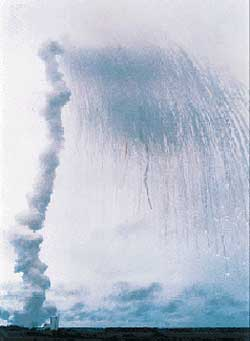
\includegraphics[width = 3.8cm]{./fig/ariane.jpg}
\end{figure}
\end{columns}
\end{frame}

\begin{frame}[fragile]
\frametitle{Pour simplifier...}
\begin{itemize}
\setlength\itemsep{2em}
\item Le type \bvrb|float| permet de repr�senter 7 d�cimales.
\item Le type \bvrb|double| permet de repr�senter 16 d�cimales.
\end{itemize}
Sans prendre en compte l'exposant,

\end{frame}
% !TEX encoding = IsoLatin9

%%%%%%%%%%%%%%%%%%%%% SECTION 1
\section{Le perceptron}
\begin{frame}
  \begin{columns}
    \column{4.8cm}
    \tableofcontents[currentsection,hideothersubsections]
    \column{7cm}
      \centering{
      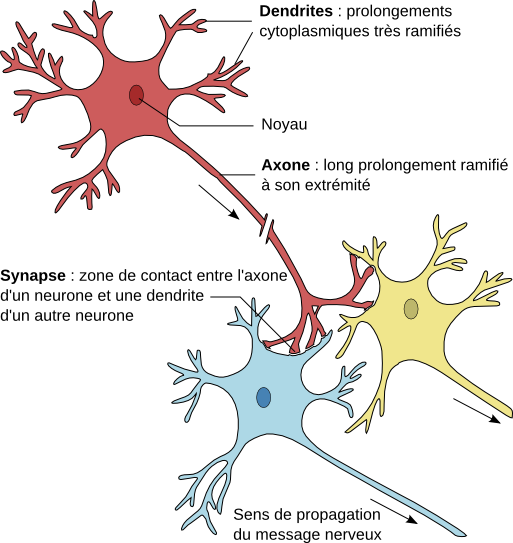
\includegraphics[width=6cm]{fig/neurone.png}
    }
  \end{columns}
  
\end{frame}


\begin{frame}
  \frametitle{Le perceptron : un neurone articiel}
  \begin{tikzpicture}[
    basic/.style={draw,fill=blue!20,text width=1em,text badly centered},
    input/.style={basic,circle},
    weights/.style={basic,rectangle},
functions/.style={basic,circle,fill=blue!10},
]
        \node[functions] (center) {};
        \node[below of=center,font=\scriptsize,text width=4em] {Fonction d'activation};
        \draw[thick] (0.5em,0.5em) -- (0,0.5em) -- (0,-0.5em) -- (-0.5em,-0.5em);
      %  \draw (0em,0.75em) -- (0em,-0.75em);
      %  \draw (0.75em,0em) -- (-0.75em,0em);
        \node[right of=center, anchor = west] (right) {$y=$ 0 ou 1};
            \path[draw,->] (center) -- (right);
        \node[functions,left=3em of center] (left) {$\sum$};
            \path[draw,->] (left) -- (center);
%        \node[weights,left=3em of left] (2) {$w_2$} -- (2) 
            \node[input,left= 4em of left] (l2) {$x_2$};
%            \path[draw,->] (l2) -- (2);
            \path[draw,->] (l2) -- node[above,midway]{$w_2$}(left);
        \node[below of=l2] (dots) {$\vdots$} ;
%(dots) node[left of=dots] (ldots) {$\vdots$};
%        \node[weights,below of=dots] (n) {$w_n$} -- (n) 
\node[input,below of=dots] (ln) {$x_n$};
%            \path[draw,->] (ln) -- (n);
            \path[draw,->] (ln) -- node[above,midway]{$w_n$}(left);
%        \node[weights,above of=2] (1) {$w_1$} -- (1) 
            \node[input,above of=l2] (l1) {$x_1$};
%            \path[draw,->] (l1) -- (1);
            \path[draw,->] (l1) -- node[above,midway]{$w_1$}(left);
%        \node[weights,above of=1] (0) {$w_0$} -- (0) 
\node[input,above of=l1] (l0) {$1$};
%            \path[draw,->] (l0) -- (0);
            \path[draw,->] (l0) -- node[above,midway]{$w_0$}(left);
        \node[below of=ln,font=\scriptsize](lin) {inputs};
        \node[right of=lin,font=\scriptsize] {weights};
    \end{tikzpicture}
\begin{block}{}
Si $w_0 + w_1\times x_1 + w_2\times x_2 +  \dots + w_n\times x_n < 0$, $\mathbf{y=0}$\\
sinon $\mathbf{y=1}$
\end{block}

\end{frame}

\begin{frame}[fragile]
\frametitle{En C, une structure de donn�es}
\begin{codeblock}{}
\vspace{-.3cm}
\lstset{escapeinside={��}}
%\lstset{basicstyle=\scriptsize}
\begin{codeC}
struct perceptron {
  short X[N] ; //entr�es
  short Y ; //sorties
  int W[N+1] ; //poids
  } ;
  
void active (struct perceptron *p) ;
\end{codeC}
\vspace{-.3cm}
\end{codeblock}
\end{frame}




\end{document} 

%%%%%%%%%%%%%%%%%%%%% SECTION 1
\section{Les algorithmes}\label{section:1}
\begin{frame}
\begin{columns}
        \column{4.8cm}
            \tableofcontents[currentsection]
        \column{7cm}
        \centering{
            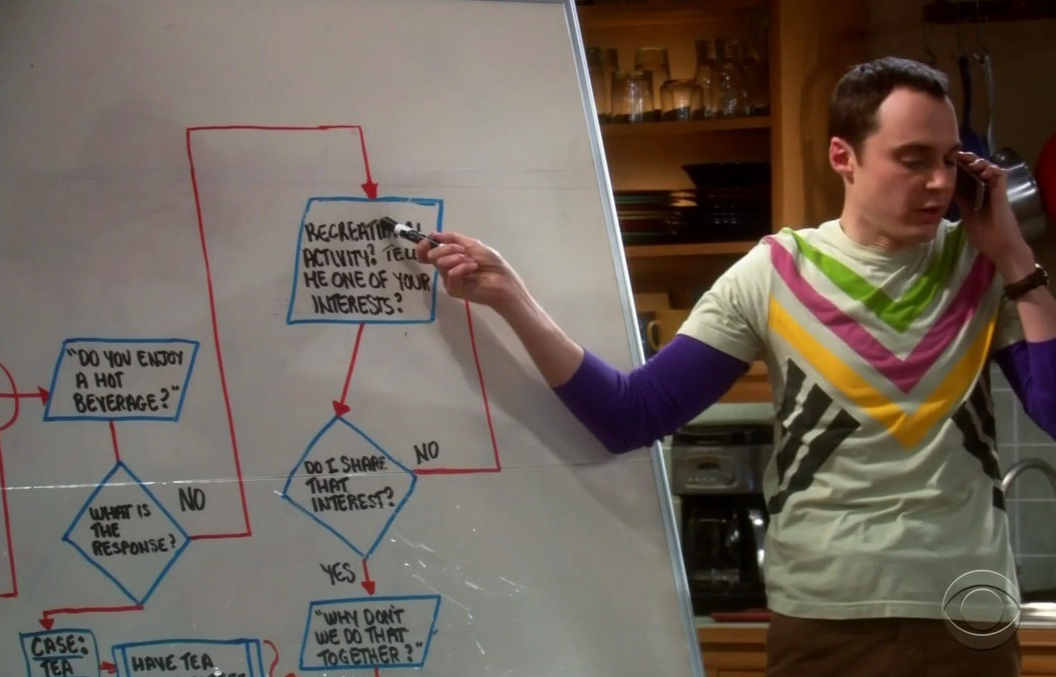
\includegraphics[width=7cm]{fig/Algorithm-sheldon.png}
            }
                 \textit{ I believe I've isolateblblblblblblsblbslbslbsl
            sblbslblsblsblblsblbs
            lbslblbslsb d the algorithm for making friends.}
     
            
            \small{
            \hfill Sheldon Cooper, 
            
            \hfill in \textit{The Big Band Theory}, Season 2, Episode 13
            }


    \end{columns}

\end{frame}


%%%%%%%%%%%%%%%%%%%%%
\subsection{Introduction}
    \begin{frame}
    \frametitle{Pourquoi faire appel � des algorithmes ?}
    Pour automatiser des t�ches
    
    Exemples :
    \begin{itemize}
    \item M�tier � tisser\\
    \item M�thode de calcul � la main d'une division\\
    \item Recette de cuisine\\
    \item ...\\
    \end{itemize}
    \end{frame}
 
 %%%%%%%%%%%%%%%%%
 
    \begin{frame}
    \frametitle{Qu'est-ce qu'un algorithme ?}
    \begin{block}{D�finition}
    Un algorithme est un ensemble 
    ordonn� d'instructions simples
permettant de r�soudre un probl�me.
    \end{block}
    \end{frame}
    
 %%%%%%%%%%%%%%%%%%
 \subsection{Construction d'un algorithme}
%%%%%%%%%%%%%%%%%%%    
\section{La machine de Turing}
%%%%%%%%%%%%%%%%%%%%
 
  
\begin{frame}[fragile]
\frametitle{Un peu d'histoire...}
\begin{codeblock}{Test}
\begin{codeC}
for (int i = 0 ; i < n ; i ++) {
    //a comment
    printf("%d",i);
    }
\end{codeC}
\end{codeblock}

\begin{termblock}{test 2}
\lstset{escapeinside={��}}
\begin{lstlisting}
�\textbf{>>}�./a.out
�\color{darkgray}{\texttt{  Hello World}}�
\end{lstlisting}
\end{termblock}

 \begin{block}{Bloc standard}
blablabla
\end{block}
\end{frame}


\begin{frame}[fragile]
\frametitle{essai}
\begin{columns}
\column{6cm}
\begin{block}

\begin{figure}
\begin{tikzpicture} [
    auto,
    decision/.style = { diamond, draw=blue, thick, fill=blue!20,
                        text width=5em, text badly centered,
                        inner sep=1pt, rounded corners },
    block/.style    = { rectangle, draw=blue, thick, 
                        fill=blue!20, text width=10em, text centered,
                        rounded corners, minimum height=2em },
    line/.style     = { draw, thick, ->, shorten >=2pt },
  ]
   \matrix [column sep=-10mm, row sep=10mm] {
                    & \node [text centered] (x) {$\mathbf{X}$};            & \\
                    & \node (null1) {};                                    & \\
                    & \node [block] (doa) {\textsf{DoAE}($\mathbf{X}$)};   & \\
  	               \node(null3){}; & \node [decision] (uiddes)
                        {\textsf{UID}($\hat{\mathbf{X}}$)};
                                  & \node[text centered](tra){$\mathbf{i}$}; \\
                  & \node [block] (track) {\textsf{DoAT}($\mathbf{x}$)}; & \\
                    & \node [block] (pesos)
                        {\textsf{BF}(DoA$_{\mathrm{T}}$,DoAs)};            & \\
                    & \node [block] (filtrado)
                        {\textsf{SF}($\mathbf{w}$,$\mathbf{x}$)};          & \\
                    & \node [text centered] (xf) {$\hat{x}(t)$ };          & \\
  };
  % connect all nodes defined above
 \begin{scope} [every path/.style=line]
    \path (x)        --    (doa);
    \path (doa)      --    node [near start] {DoAs} (uiddes);
    \path (tra)      --    (uiddes);
    \path (uiddes)   --++  (-3,0) node [near start] {no} |- (null1);
    \path (uiddes)   --    node [near start] {DoA} (track);
    \path (track)    --    node [near start] {DoA$_{\mathrm{T}}$} (pesos);
    \path (pesos)    --    node [near start] {\textbf{w}} (filtrado);
    \path (filtrado) --    (xf);
  
  \end{scope}
\end{tikzpicture}
\end{figure}
\end{block}
\column{3cm}
\begin{block}{bulbul}
\end{block}
\end{columns}
\end{frame}

\end{document}
